\documentclass[11pt]{ctexart}
\usepackage[a4paper,margin=1in]{geometry}
\usepackage{amsmath,amssymb,amsfonts}
\usepackage{booktabs}
\usepackage{graphicx}
\usepackage{caption}
\usepackage{enumitem}
\usepackage{pgfplots}
\usepackage{pgfplotstable}
\usepackage{tikz}
\usepackage[hidelinks]{hyperref}
\usepackage{microtype}
\setlength{\emergencystretch}{4em}

\usetikzlibrary{calc,arrows.meta}
\pgfplotsset{compat=1.18}
\definecolor{accentA}{RGB}{31,119,180}
\definecolor{accentB}{RGB}{255,127,14}
\definecolor{accentC}{RGB}{44,160,44}
\definecolor{accentD}{RGB}{148,103,189}
\definecolor{accentE}{RGB}{214,39,40}
\pgfplotscreateplotcyclelist{accentcolors}{
{accentA, thick},
{accentB, thick},
{accentC, thick},
{accentD, thick},
{accentE, thick}
}
\pgfplotsset{
  fptaxis/.style={
    width=\linewidth,
    height=4.8cm,
    scale only axis,
    xlabel={$t$},
    ylabel={$f(t)$},
    grid=both,
    major grid style={line width=0.35pt, draw=gray!25},
    minor grid style={line width=0.2pt, draw=gray!15},
    axis line style={black!60},
    tick align=outside,
    tick style={black!60},
    label style={font=\small},
    ticklabel style={font=\footnotesize},
    legend style={font=\scriptsize, draw=none, fill=none},
    cycle list name=accentcolors,
    unbounded coords=jump,
  },
  fptaxislin/.style={
    width=0.78\linewidth,
    height=4.6cm,
    scale only axis,
    xlabel={$t$},
    ylabel={$f(t)$},
    grid=major,
    major grid style={line width=0.35pt, draw=gray!20},
    axis background/.style={fill=gray!3},
    axis line style={black!60},
    tick align=outside,
    tick style={black!60},
    label style={font=\small},
    ticklabel style={font=\footnotesize},
    title style={font=\small},
    legend style={font=\scriptsize, draw=none, fill=none},
    cycle list name=accentcolors,
    unbounded coords=jump,
    line cap=round,
    line join=round,
  },
  scanaxis/.style={
    width=\linewidth,
    height=4.8cm,
    scale only axis,
    view={0}{90},
    colormap={bimodal}{rgb=(0.95,0.95,0.95) rgb=(0.50,0.80,0.72) rgb=(0.98,0.70,0.48)},
    point meta min=0,
    point meta max=2,
    axis line style={black!60},
    tick align=outside,
    tick style={black!60},
    label style={font=\small},
    ticklabel style={font=\footnotesize},
  },
}

\newcommand{\configcard}[1]{%
  \vspace{-6pt}%
  \noindent\makebox[\linewidth][c]{%
    \fcolorbox{gray!35}{gray!6}{%
      \begin{minipage}{0.88\linewidth}%
        \scriptsize\raggedright%
        \renewcommand{\arraystretch}{0.9}%
        #1%
      \end{minipage}%
    }%
  }%
}

\newcommand{\ringcaseNoSc}[4]{%
  \def\N{#1}\def\start{#2}\def\tone{#3}\def\ttwo{#4}\def\R{1.0}%
  \coordinate (C) at (0,0);%
  \pgfmathsetmacro{\angStart}{360*\start/\N}%
  \pgfmathsetmacro{\angTone}{360*\tone/\N}%
  \pgfmathsetmacro{\angTtwo}{360*\ttwo/\N}%
  \coordinate (S) at ({\R*cos(\angStart)},{\R*sin(\angStart)});%
  \coordinate (T1) at ({\R*cos(\angTone)},{\R*sin(\angTone)});%
  \coordinate (T2) at ({\R*cos(\angTtwo)},{\R*sin(\angTtwo)});%
  \draw[gray!60,line width=0.9pt] (C) circle (\R);%
  \fill[accentE] (S) circle (0.022);%
  \fill[accentA] (T1) circle (0.022);%
  \fill[accentA] (T2) circle (0.022);%
  \node[font=\scriptsize, text=accentE] at ($(C)!1.25!(S)$) {s};%
  \node[font=\scriptsize, text=accentA] at ($(C)!1.23!(T1)$) {t1};%
  \node[font=\scriptsize, text=accentA] at ($(C)!1.23!(T2)$) {t2};%
}

\newcommand{\ringcaseSc}[6]{%
  \def\N{#1}\def\start{#2}\def\tone{#3}\def\ttwo{#4}\def\src{#5}\def\dst{#6}\def\R{1.0}%
  \coordinate (C) at (0,0);%
  \pgfmathsetmacro{\angStart}{360*\start/\N}%
  \pgfmathsetmacro{\angTone}{360*\tone/\N}%
  \pgfmathsetmacro{\angTtwo}{360*\ttwo/\N}%
  \pgfmathsetmacro{\angSrc}{360*\src/\N}%
  \pgfmathsetmacro{\angDst}{360*\dst/\N}%
  \coordinate (S) at ({\R*cos(\angStart)},{\R*sin(\angStart)});%
  \coordinate (T1) at ({\R*cos(\angTone)},{\R*sin(\angTone)});%
  \coordinate (T2) at ({\R*cos(\angTtwo)},{\R*sin(\angTtwo)});%
  \coordinate (U) at ({\R*cos(\angSrc)},{\R*sin(\angSrc)});%
  \coordinate (V) at ({\R*cos(\angDst)},{\R*sin(\angDst)});%
  \draw[gray!60,line width=0.9pt] (C) circle (\R);%
  \fill[accentE] (S) circle (0.022);%
  \fill[accentA] (T1) circle (0.022);%
  \fill[accentA] (T2) circle (0.022);%
  \fill[accentB] (U) circle (0.02);%
  \draw[accentC,line width=0.9pt] (V) circle (0.03);%
  \node[font=\scriptsize, text=accentE] at ($(C)!1.25!(S)$) {s};%
  \node[font=\scriptsize, text=accentA] at ($(C)!1.23!(T1)$) {t1};%
  \node[font=\scriptsize, text=accentA] at ($(C)!1.23!(T2)$) {t2};%
  \node[font=\scriptsize, text=accentB] at ($(C)!1.23!(U)$) {src};%
  \node[font=\scriptsize, text=accentC] at ($(C)!1.23!(V)$) {dst};%
  \draw[->,accentC,line width=1.0pt] (U) to[out=40,in=20,looseness=1.3] (V);%
}

\newcommand{\ringcaseScOverlap}[6]{%
  \def\N{#1}\def\start{#2}\def\tone{#3}\def\ttwo{#4}\def\src{#5}\def\dst{#6}\def\R{1.0}%
  \coordinate (C) at (0,0);%
  \pgfmathsetmacro{\angStart}{360*\start/\N}%
  \pgfmathsetmacro{\angTone}{360*\tone/\N}%
  \pgfmathsetmacro{\angTtwo}{360*\ttwo/\N}%
  \pgfmathsetmacro{\angSrc}{360*\src/\N}%
  \pgfmathsetmacro{\angDst}{360*\dst/\N}%
  \pgfmathsetmacro{\angTtwoLab}{\angTtwo-22}%
  \pgfmathsetmacro{\angDstLab}{\angDst+26}%
  \coordinate (S) at ({\R*cos(\angStart)},{\R*sin(\angStart)});%
  \coordinate (T1) at ({\R*cos(\angTone)},{\R*sin(\angTone)});%
  \coordinate (T2) at ({\R*cos(\angTtwo)},{\R*sin(\angTtwo)});%
  \coordinate (U) at ({\R*cos(\angSrc)},{\R*sin(\angSrc)});%
  \coordinate (V) at ({\R*cos(\angDst)},{\R*sin(\angDst)});%
  \draw[gray!60,line width=0.9pt] (C) circle (\R);%
  \fill[accentE] (S) circle (0.022);%
  \fill[accentA] (T1) circle (0.022);%
  \fill[accentA] (T2) circle (0.022);%
  \fill[accentB] (U) circle (0.02);%
  \draw[accentC,line width=0.9pt] (V) circle (0.03);%
  \node[font=\scriptsize, text=accentE] at ($(C)!1.25!(S)$) {s};%
  \coordinate (T1L) at ($(T1)+(-0.28,0.36)$);%
  \draw[accentA!70,line width=0.6pt] (T1) -- (T1L);%
  \node[font=\scriptsize, text=accentA] at (T1L) {t1};%
  \coordinate (T2L) at ({1.18*cos(\angTtwoLab)},{1.18*sin(\angTtwoLab)});%
  \draw[accentA!70,line width=0.6pt] (T2) -- (T2L);%
  \node[font=\scriptsize, text=accentA] at (T2L) {t2};%
  \node[font=\scriptsize, text=accentB] at ($(C)!1.23!(U)$) {src};%
  \coordinate (VLab) at ($(V)+(-0.28,-0.36)$);%
  \draw[accentC!70,line width=0.6pt] (V) -- (VLab);%
  \node[font=\scriptsize, text=accentC] at (VLab) {dst};%
  \draw[->,accentC,line width=1.0pt] (U) to[out=40,in=20,looseness=1.3] (V);%
}

\title{双目标 lazy ring：无 shortcut / 有 shortcut 的多峰首达机制与数值结果}
\author{}
\date{}

\setlist{nosep}
\setlength{\textfloatsep}{8pt plus 2pt minus 2pt}
\setlength{\floatsep}{6pt plus 2pt minus 2pt}
\setlength{\intextsep}{6pt plus 2pt minus 2pt}
\setlength{\abovecaptionskip}{4pt}
\setlength{\belowcaptionskip}{0pt}

\begin{document}
\sloppy
\maketitle

\section*{参数定义（读图对照）}
所有索引均按 $N$ 取模。正向定义为节点编号递增方向（示意图中为顺时针）。
\begin{itemize}
  \item $N$：环上节点数。
  \item $n_0$：起点。
  \item $(m_1,m_2)$：两个吸收目标。
  \item $K$：每步可走的邻居数（$K=2$ 为 $\pm1$，$K=4$ 为 $\pm1,\pm2$）。
  \item $q$：移动概率；停留概率为 $1-q$。
  \item $g$：全局漂移（偏置）参数；$g>0$ 偏向正向。
  \item $\beta$：shortcut 强度（selfloop 规则）；shortcut 概率 $p=\beta(1-q)$。
  \item $\mathrm{src},\mathrm{dst}$：shortcut 起点/终点。
  \item $\rho_k$：在目标 $m_k$ 的吸收概率（本文取 $\rho_1=\rho_2=1$）。
\end{itemize}

\section*{结论与关键图示}
我们构建了\textbf{双目标}的 lazy ring 体系，并在\textbf{无 shortcut}与\textbf{有 shortcut（selfloop 规则）}两条主线上给出可复现的双峰/三峰例子。
结论要点如下：
\begin{enumerate}
  \item \textbf{无 shortcut 但有漂移时}，双目标首达分布可稳定出现双峰：
  逆漂移短路径给出快峰，顺漂移绕行给出慢峰（图~\ref{fig:caseA}--\ref{fig:caseB}）。
  \item \textbf{有 shortcut 时}，双目标首达分布呈现典型的“快/慢通道”叠加；
  快峰由 shortcut 通道主导，慢峰由非 shortcut 通道主导，并在 $(N,\beta)$ 平面上形成双峰窗口（图~\ref{fig:caseC}--\ref{fig:caseD}，图~\ref{fig:scan}）。
  \item \textbf{三峰示例}可由强漂移 + $K=4$ 的 jump-over 机制触发，出现按“圈数”分层的多峰列（图~\ref{fig:caseE}）。
\end{enumerate}

\begin{figure}[!htbp]
  \centering
  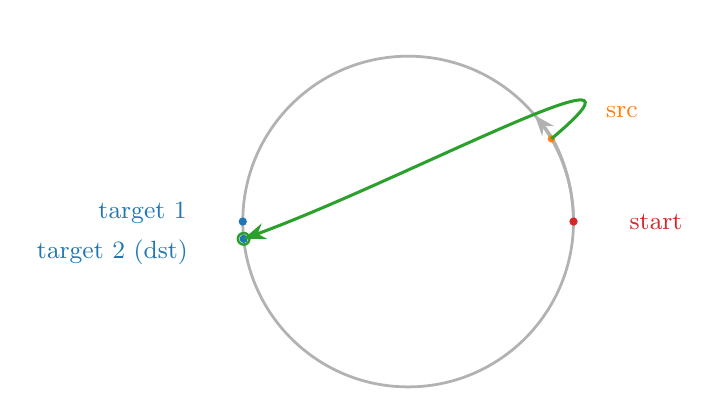
\begin{tikzpicture}[scale=2.1, >=Stealth]
    \def\N{60}
    \def\start{0}
    \def\tone{30}
    \def\ttwo{31}
    \def\src{5}
    \def\R{1.0}
    \coordinate (C) at (0,0);
    \pgfmathsetmacro{\angStart}{360*\start/\N}
    \pgfmathsetmacro{\angTone}{360*\tone/\N}
    \pgfmathsetmacro{\angTtwo}{360*\ttwo/\N}
    \pgfmathsetmacro{\angSrc}{360*\src/\N}
    \coordinate (S) at ({\R*cos(\angStart)},{\R*sin(\angStart)});
    \coordinate (T1) at ({\R*cos(\angTone)},{\R*sin(\angTone)});
    \coordinate (T2) at ({\R*cos(\angTtwo)},{\R*sin(\angTtwo)});
    \coordinate (U) at ({\R*cos(\angSrc)},{\R*sin(\angSrc)});

    \draw[gray!60,line width=1.0pt] (C) circle (\R);
    \draw[->,gray!60,line width=1.0pt] (\R,0) arc (0:40:\R);

    \fill[accentE] (S) circle (0.025);
    \fill[accentA] (T1) circle (0.025);
    \fill[accentA] (T2) circle (0.025);
    \draw[accentC,line width=0.9pt] (T2) circle (0.035);
    \fill[accentB] (U) circle (0.022);

    \node[anchor=west, font=\small, text=accentE] at ($(C)!1.28!(S)$) {start};
    \node[anchor=east, font=\small, text=accentA] at ($(C)!1.28!(T1)+(0,0.05)$) {target 1};
    \node[anchor=east, font=\small, text=accentA] at ($(C)!1.28!(T2)+(0,-0.05)$) {target 2 (dst)};
    \node[anchor=west, font=\small, text=accentB] at ($(C)!1.28!(U)+(0.03,0.02)$) {src};

    \draw[->,accentC,line width=1.1pt] (U) to[out=40,in=20,looseness=1.35] (T2);
  \end{tikzpicture}
  \caption{双目标 lazy ring + 单向 shortcut 的几何示意（报告中的 shortcut 案例参数）。}
  \label{fig:geometry}
\end{figure}

\paragraph{明确配置（所有下标按 $N$ 取模）。}
起点固定为 $n_0=0$。代表性案例的两目标与 shortcut 配置如下：
\begin{itemize}
  \item \textbf{Case A（无 shortcut，$K=2$）:} $N=20$，目标 $(m_1,m_2)=(18,10)$，$q=2/3$，$g=0.6$，$\beta=0$。
  \item \textbf{Case B（无 shortcut，$K=4$）:} $N=30$，目标 $(m_1,m_2)=(27,15)$，$q=2/3$，$g=0.6$，$\beta=0$。
  \item \textbf{Case C/D（有 shortcut，$K=2/4$）:} $N=60$，目标 $(m_1,m_2)=(30,31)$，$\mathrm{src}=5$，$\mathrm{dst}=31$，
  $q=2/3$，$g=0$，$\beta=0.02$。
  \item \textbf{Case E（三峰，无 shortcut，$K=4$）:} $N=30$，目标 $(m_1,m_2)=(29,20)$，$q=0.9$，$g=0.8$，$\beta=0$。
\end{itemize}
同样配置已汇总在表~\ref{tab:configs}。

\section*{代表性 case：几何 + FPT}
\begin{figure}[!htbp]
  \centering
  \begin{minipage}{0.24\linewidth}
    \centering
    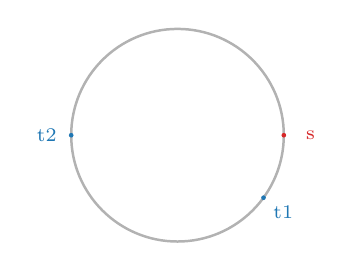
\begin{tikzpicture}[scale=1.35]
      \ringcaseNoSc{20}{0}{18}{10}
    \end{tikzpicture}
  \end{minipage}%
  \hfill
  \begin{minipage}{0.72\linewidth}
    \centering
    \begin{tikzpicture}
      \begin{axis}[
        fptaxislin,
        xmin=0, xmax=60,
        ymin=0, ymax=0.06,
        title={Case A：无 shortcut（$K=2$, $g=0.6$）},
      ]
        \addplot[accentA, very thick] table [x=t, y=f_total, col sep=comma] {outputs/A_no_sc_K2_fpt.csv};
        \addplot[black!35, dashed] coordinates {(2,0) (2,0.06)};
        \addplot[black!35, dashed] coordinates {(20,0) (20,0.06)};
        \addplot[only marks, mark=*, mark size=1.6, accentB]
          coordinates {(2,0.0177778) (20,0.0529520)};
        \node[font=\scriptsize, fill=white, fill opacity=0.85, text opacity=1, inner sep=1pt, xshift=6pt, yshift=8pt]
          at (axis cs:2,0.0177778) {$t_1=2$};
        \node[font=\scriptsize, fill=white, fill opacity=0.85, text opacity=1, inner sep=1pt, xshift=-6pt, yshift=8pt]
          at (axis cs:20,0.0529520) {$t_2=20$};
      \end{axis}
    \end{tikzpicture}
  \end{minipage}
  \caption{Case A：几何与双峰 FPT（圆点为峰值，虚线为 $t_1,t_2$）。}
  \label{fig:caseA}
\end{figure}

\begin{figure}[!htbp]
  \centering
  \begin{minipage}{0.24\linewidth}
    \centering
    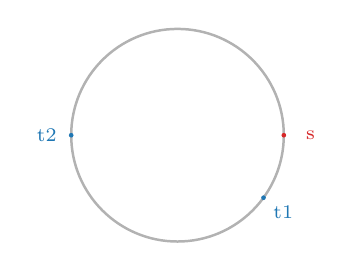
\begin{tikzpicture}[scale=1.35]
      \ringcaseNoSc{30}{0}{27}{15}
    \end{tikzpicture}
  \end{minipage}%
  \hfill
  \begin{minipage}{0.72\linewidth}
    \centering
    \begin{tikzpicture}
      \begin{axis}[
        fptaxislin,
        xmin=0, xmax=60,
        ymin=0, ymax=0.045,
        title={Case B：无 shortcut（$K=4$, $g=0.6$）},
      ]
        \addplot[accentA, very thick] table [x=t, y=f_total, col sep=comma] {outputs/B_no_sc_K4_fpt.csv};
        \addplot[black!35, dashed] coordinates {(3,0) (3,0.045)};
        \addplot[black!35, dashed] coordinates {(20,0) (20,0.045)};
        \addplot[only marks, mark=*, mark size=1.6, accentB]
          coordinates {(3,0.0097778) (20,0.0373013)};
        \node[font=\scriptsize, fill=white, fill opacity=0.85, text opacity=1, inner sep=1pt, xshift=6pt, yshift=8pt]
          at (axis cs:3,0.0097778) {$t_1=3$};
        \node[font=\scriptsize, fill=white, fill opacity=0.85, text opacity=1, inner sep=1pt, xshift=-6pt, yshift=8pt]
          at (axis cs:20,0.0373013) {$t_2=20$};
      \end{axis}
    \end{tikzpicture}
  \end{minipage}
  \caption{Case B：几何与双峰 FPT（圆点为峰值，虚线为 $t_1,t_2$）。}
  \label{fig:caseB}
\end{figure}

\begin{figure}[!htbp]
  \centering
  \begin{minipage}{0.24\linewidth}
    \centering
    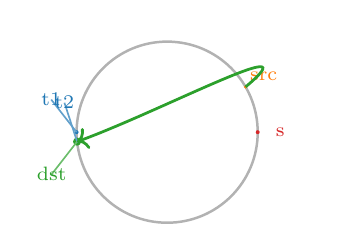
\begin{tikzpicture}[scale=1.15]
      \ringcaseScOverlap{60}{0}{30}{31}{5}{31}
    \end{tikzpicture}
  \end{minipage}%
  \hfill
  \begin{minipage}{0.72\linewidth}
    \centering
    \begin{tikzpicture}
      \begin{axis}[
        fptaxislin,
        xmin=0, xmax=500,
        ymin=0, ymax=0.0010,
        title={Case C：有 shortcut（$K=2$, $\beta=0.02$）},
      ]
        \addplot[accentA, very thick] table [x=t, y=f_total, col sep=comma] {outputs/C_sc_K2_fpt.csv};
        \addplot[black!35, dashed] coordinates {(36,0) (36,0.0010)};
        \addplot[black!35, dashed] coordinates {(387,0) (387,0.0010)};
        \addplot[only marks, mark=*, mark size=1.6, accentB]
          coordinates {(36,0.000313811) (387,0.000801570)};
        \node[font=\scriptsize, fill=white, fill opacity=0.85, text opacity=1, inner sep=1pt, xshift=6pt, yshift=8pt]
          at (axis cs:36,0.000313811) {$t_1=36$};
        \node[font=\scriptsize, fill=white, fill opacity=0.85, text opacity=1, inner sep=1pt, xshift=-6pt, yshift=8pt]
          at (axis cs:387,0.000801570) {$t_2=387$};
      \end{axis}
    \end{tikzpicture}
  \end{minipage}
  \caption{Case C：几何与双峰 FPT（圆点为峰值，虚线为 $t_1,t_2$）。}
  \label{fig:caseC}
\end{figure}

\begin{figure}[!htbp]
  \centering
  \begin{minipage}{0.24\linewidth}
    \centering
    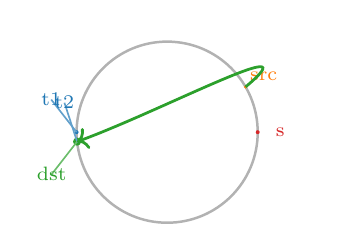
\begin{tikzpicture}[scale=1.15]
      \ringcaseScOverlap{60}{0}{30}{31}{5}{31}
    \end{tikzpicture}
  \end{minipage}%
  \hfill
  \begin{minipage}{0.72\linewidth}
    \centering
    \begin{tikzpicture}
      \begin{axis}[
        fptaxislin,
        xmin=0, xmax=250,
        ymin=0, ymax=0.0022,
        title={Case D：有 shortcut（$K=4$, $\beta=0.02$）},
      ]
        \addplot[accentA, very thick] table [x=t, y=f_total, col sep=comma] {outputs/D_sc_K4_fpt.csv};
        \addplot[black!35, dashed] coordinates {(15,0) (15,0.0022)};
        \addplot[black!35, dashed] coordinates {(169,0) (169,0.0022)};
        \addplot[only marks, mark=*, mark size=1.6, accentB]
          coordinates {(15,0.000319354) (169,0.00183952)};
        \node[font=\scriptsize, fill=white, fill opacity=0.85, text opacity=1, inner sep=1pt, xshift=6pt, yshift=8pt]
          at (axis cs:15,0.000319354) {$t_1=15$};
        \node[font=\scriptsize, fill=white, fill opacity=0.85, text opacity=1, inner sep=1pt, xshift=-6pt, yshift=8pt]
          at (axis cs:169,0.00183952) {$t_2=169$};
      \end{axis}
    \end{tikzpicture}
  \end{minipage}
  \caption{Case D：几何与双峰 FPT（圆点为峰值，虚线为 $t_1,t_2$）。}
  \label{fig:caseD}
\end{figure}

\begin{figure}[!htbp]
  \centering
  \begin{minipage}{0.26\linewidth}
    \centering
    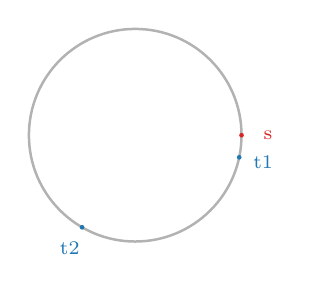
\begin{tikzpicture}[scale=1.35]
      \ringcaseNoSc{30}{0}{29}{20}
    \end{tikzpicture}
  \end{minipage}\hfill
  \begin{minipage}{0.70\linewidth}
    \centering
    \begin{tikzpicture}
      \begin{axis}[
        fptaxislin,
        xmin=0, xmax=90,
        ymin=0, ymax=0.08,
        title={Case E：三峰（$K=4$, $g=0.8$）},
      ]
        \addplot[accentA, very thick] table [x=t, y=f_total, col sep=comma] {outputs/E_triple_K4_fpt.csv};
        \addplot[black!35, dashed] coordinates {(1,0) (1,0.08)};
        \addplot[black!35, dashed] coordinates {(17,0) (17,0.08)};
        \addplot[black!35, dashed] coordinates {(43,0) (43,0.08)};
        \addplot[only marks, mark=*, mark size=1.6, accentB]
          coordinates {(1,0.045) (17,0.0704637) (43,0.00417010)};
        \node[font=\scriptsize, fill=white, fill opacity=0.85, text opacity=1, inner sep=1pt, xshift=6pt, yshift=8pt]
          at (axis cs:1,0.045) {$t_1=1$};
        \node[font=\scriptsize, fill=white, fill opacity=0.85, text opacity=1, inner sep=1pt, xshift=6pt, yshift=8pt]
          at (axis cs:17,0.0704637) {$t_2=17$};
        \node[font=\scriptsize, fill=white, fill opacity=0.85, text opacity=1, inner sep=1pt, xshift=-6pt, yshift=8pt]
          at (axis cs:43,0.00417010) {$t_3=43$};
      \end{axis}
    \end{tikzpicture}
  \end{minipage}
  \caption{Case E：几何与三峰 FPT（圆点为峰值，虚线为峰位置）。}
  \label{fig:caseE}
\end{figure}

\section*{模型与数学机理（双目标吸收）}
\paragraph{Lazy ring 与漂移。}
环上有 $N$ 个节点（$0,1,\dots,N-1$）。每步以概率 $1-q$ 停留，以概率 $q$ 在环上移动。
对 $K=2$（位移 $\pm 1$）与 $K=4$（位移 $\pm1,\pm2$），引入漂移参数 $g\in[-1,1]$：
\begin{align}
  P(+)=\frac{q(1+g)}{2},\qquad P(-)=\frac{q(1-g)}{2},
\end{align}
并在同向步长之间均分概率（例如 $K=4$ 时 $+1,+2$ 各取 $P(+)/2$）。

\paragraph{Shortcut（selfloop 规则）。}
仅在源点 $\mathrm{src}$ 处，把自环概率的一部分挪到 $\mathrm{src}\to\mathrm{dst}$：
\begin{align}
  p=\beta(1-q),\qquad P(\mathrm{src}\to\mathrm{src})=1-q-p,\qquad P(\mathrm{src}\to\mathrm{dst})=p.
\end{align}
其余节点与无 shortcut 情形一致。

\paragraph{两目标吸收的精确递推。}
设目标为 $m_1,m_2$，到达任一目标即吸收。令 $\mathbf{p}_t$ 为“吸收后”的分布，则
\begin{align}
  \mathbf{p}_{t+1}=\mathbf{p}_t\mathbf{W},\qquad
  f_i(t+1)=[\mathbf{p}_{t+1}]_{m_i},\qquad
  \mathbf{p}_{t+1}(m_i)=0,\ i\in\{1,2\}.
\end{align}
因此总首达分布为 $f(t)=f_1(t)+f_2(t)$，生存函数
$S(t)=\sum_i p_t(i)$ 满足 $S(t+1)=S(t)-f(t+1)$。

\paragraph{吸收马尔可夫链视角。}
将转移矩阵写成
\begin{align}
\mathbf{W}=\begin{pmatrix}\mathbf{Q} & \mathbf{R}\\ 0 & I\end{pmatrix},
\end{align}
其中 $\mathbf{Q}$ 是“非吸收态”子链，$\mathbf{R}$ 给出一步进入两个吸收点的概率。
令 $\mathbf{r}_i$ 是 $\mathbf{R}$ 中对应目标 $m_i$ 的列，初始分布为 $\mathbf{p}_0$，则
\begin{align}
  f_i(t+1)=\mathbf{r}_i^{\mathsf T}\mathbf{Q}^{t}\mathbf{p}_0,\qquad
  f(t+1)=\mathbf{r}^{\mathsf T}\mathbf{Q}^{t}\mathbf{p}_0,
\end{align}
其中 $\mathbf{r}=\mathbf{r}_1+\mathbf{r}_2$。生成函数形式为
\begin{align}
  \widetilde f_i(z)=z\,\mathbf{r}_i^{\mathsf T}(I-z\mathbf{Q})^{-1}\mathbf{p}_0.
\end{align}
等价地，生存函数为
\begin{align}
  S(t)=\mathbf{1}^{\mathsf T}\mathbf{Q}^{t}\mathbf{p}_0,\qquad f(t+1)=S(t)-S(t+1),
\end{align}
因此两目标首达完全由 $\mathbf{Q}$ 与两列 $\mathbf{r}_1,\mathbf{r}_2$ 决定。
若 $\mathbf{Q}$ 可对角化，$\mathbf{Q}=\mathbf{V}\mathbf{\Lambda}\mathbf{V}^{-1}$，
则
\begin{align}
  f(t+1)=\sum_k c_k\,\lambda_k^{\,t},
\end{align}
多个时间尺度（不同 $|\lambda_k|$）的模态权重可比时就会出现多峰。
这给出了“\textbf{两目标吸收的完整数学机制}”：
时间域上是 $\mathbf{Q}$ 的幂次叠加，频域上是 $(I-z\mathbf{Q})^{-1}$ 的谱结构。

\paragraph{与 Giuggioli 多目标公式的对应。}
对任意图上的随机游走，单目标首达生成函数满足
\begin{align}
  \widetilde F_{i\to j}(z)=\frac{\widetilde P_i(j;z)}{\widetilde P_j(j;z)}.
\end{align}
两目标 splitting 首达可写为 $2\times2$ 行列式比值\cite{giuggioli2023}：若
$G_k=\widetilde F_{n_0\to m_k}(z)$，
$F_{jk}$ 由目标间首达与回返项组成，则
\begin{align}
\widetilde F_{n_0\to (m_1\mid m_2)}(z)=\frac{G_1F_{22}-F_{12}G_2}{F_{11}F_{22}-F_{12}F_{21}},
\end{align}
另一目标对称可得，总首达为两者相加。
对部分吸收 $\rho_k$，对角元为
\begin{align}
  F_{kk}=1+\frac{1-\rho_k}{\rho_k}\,[1-R_{m_k}(z)],
\end{align}
其中 $R_{m_k}(z)$ 表示在不被另一目标吸收的条件下回到 $m_k$ 的生成函数。
在本报告的 $\rho_1=\rho_2=1$ 情形下，$F_{11}=F_{22}=1$，公式进一步简化。

\paragraph{多峰机理（直观图像）。}
多峰来自\textbf{多条路径族/多时间尺度的叠加}：
漂移会分裂为“逆漂移快峰”与“顺漂移慢峰”；
shortcut 会分裂为“用 shortcut 的快通道”与“未用 shortcut 的慢通道”；
两目标进一步对概率质量做 splitting，从而放大峰的可见性。

\section*{无 shortcut：漂移驱动的双峰}
Case A/B（图~\ref{fig:caseA}--\ref{fig:caseB}）给出无 shortcut 情形的双峰示例，
图~\ref{fig:splitting} 显示两目标分裂后的贡献。

\begin{figure}[!htbp]
  \centering
  \begin{tikzpicture}
    \begin{semilogyaxis}[
      fptaxis,
      width=0.86\linewidth,
      title={splitting by targets (no shortcut, $K=2$)},
      xmin=0, xmax=140,
      ymin=1e-12, ymax=1,
      legend style={at={(0.02,0.98)}, anchor=north west},
    ]
      \addplot[black!70, thick] table [x=t, y=f_total, col sep=comma] {outputs/A_no_sc_K2_fpt.csv};
      \addplot[accentC, dashed] table [x=t, y=f_target1, col sep=comma] {outputs/A_no_sc_K2_fpt.csv};
      \addplot[accentB, dashed] table [x=t, y=f_target2, col sep=comma] {outputs/A_no_sc_K2_fpt.csv};
      \legend{total,target 1,target 2}
    \end{semilogyaxis}
  \end{tikzpicture}
  \caption{两目标 splitting：总 FPT=目标1分量+目标2分量。}
  \label{fig:splitting}
\end{figure}

\section*{有 shortcut：快/慢通道叠加}
Case C/D（图~\ref{fig:caseC}--\ref{fig:caseD}）展示 selfloop 规则下的双峰例子（$K=2$ 与 $K=4$）。
图~\ref{fig:scan} 给出 $(N,\beta)$ 的双峰相图（0=无双峰，1=paper 双峰，2=macro 双峰）。

\begin{figure}[!htbp]
  \centering
  \begin{minipage}{0.45\linewidth}
    \centering
    \textbf{(a) $K=2$}\par
    \begin{tikzpicture}
      \begin{axis}[
        scanaxis,
        width=0.76\linewidth,
        xlabel={$\beta$}, ylabel={$N$},
        title={bimodality map},
        mesh/cols=9,
      ]
        \addplot[matrix plot*, point meta=explicit]
          table [x=beta, y=N, meta=flag, col sep=comma] {data/scan_bimodality_K2.csv};
      \end{axis}
    \end{tikzpicture}
  \end{minipage}%
  \hfill
  \begin{minipage}{0.45\linewidth}
    \centering
    \textbf{(b) $K=4$}\par
    \begin{tikzpicture}
      \begin{axis}[
        scanaxis,
        width=0.76\linewidth,
        xlabel={$\beta$}, ylabel={$N$},
        title={bimodality map},
        mesh/cols=9,
      ]
        \addplot[matrix plot*, point meta=explicit]
          table [x=beta, y=N, meta=flag, col sep=comma] {data/scan_bimodality_K4.csv};
      \end{axis}
    \end{tikzpicture}
  \end{minipage}
  \caption{双峰相图（0=无双峰，1=paper，2=macro）。几何：$\mathrm{src}=5,\ \mathrm{dst}=m_2,\ m_1=\lfloor N/2\rfloor,\ m_2=m_1+1$。}
  \label{fig:scan}
\end{figure}

\section*{三峰示例}
Case E（图~\ref{fig:caseE}）展示了三峰例子：强漂移 + $K=4$ 带来的 jump-over 使得
“按圈数”的首达族群出现多峰列。

\section*{模型配置与复现}
表~\ref{tab:configs} 与表~\ref{tab:peaks} 汇总了报告中的代表性案例与峰信息。
复现命令：
\begin{verbatim}
cd reports/ring_two_target
python3 code/two_target_report.py
latexmk -xelatex -auxdir=build -emulate-aux-dir ring_two_target_cn.tex
\end{verbatim}

\begin{table}[!htbp]
  \centering
  \caption{代表性案例配置（详见 \texttt{data/model\_configs.csv}）。}
  \label{tab:configs}
  \begin{tabular}{lllllll}
\toprule
Case & $N$ & $K$ & $q$ & $g$ & $\beta$ & targets \\
\midrule
A\_no\_sc\_K2 & 20 & 2 & 0.667 & 0.60 & 0.000 & (18,10) \\
B\_no\_sc\_K4 & 30 & 4 & 0.667 & 0.60 & 0.000 & (27,15) \\
C\_sc\_K2 & 60 & 2 & 0.667 & 0.00 & 0.020 & (30,31) \\
D\_sc\_K4 & 60 & 4 & 0.667 & 0.00 & 0.020 & (30,31) \\
E\_triple\_K4 & 30 & 4 & 0.900 & 0.80 & 0.000 & (29,20) \\
\bottomrule
\end{tabular}
\end{table}

\begin{table}[!htbp]
  \centering
  \caption{峰位置与判据（$t_1$ 为最早峰，$t_2$ 为最晚峰）。}
  \label{tab:peaks}
  \begin{tabular}{llllllll}
\toprule
Case & $t_1$ & $h_1$ & $t_2$ & $h_2$ & $h_2/h_1$ & paper & macro \\
\midrule
A\_no\_sc\_K2 & 2 & 1.78e-02 & 20 & 5.30e-02 & 2.98 & True & True \\
B\_no\_sc\_K4 & 3 & 9.78e-03 & 20 & 3.73e-02 & 3.81 & True & False \\
C\_sc\_K2 & 36 & 3.14e-04 & 387 & 8.02e-04 & 2.55 & True & True \\
D\_sc\_K4 & 15 & 3.19e-04 & 169 & 1.84e-03 & 5.76 & True & True \\
E\_triple\_K4 & 1 & 4.50e-02 & 43 & 4.17e-03 & 0.09 & True & True \\
\bottomrule
\end{tabular}
\end{table}

\begin{thebibliography}{9}
\bibitem{giuggioli2023}
L. Giuggioli et al., \emph{Multi-target search in bounded and heterogeneous environments: a lattice random walk perspective}, arXiv:2311.00464v2.
\bibitem{sarvaharman2020}
A. Sarvaharman and L. Giuggioli, \emph{Phys. Rev. E} 102, 062124 (2020).
\end{thebibliography}

\end{document}
